\section{Source-Void-to-Absorber Test Problem}

In this section, results are presented for the
source-void-to-absorber test problem
described in Section \ref{sec:source_void_to_absorber}.
Table \ref{tab:source_void_to_absorber_run_parameters}
shows the run parameters used
to obtain these results, and Figure \ref{fig:source_void_to_absorber}
shows the results for this problem. Figure
\ref{fig:source_void_to_absorber_fine} shows results
for a fine mesh that illustrates the shortcomings of Galerkin-FCT
vs. EV-FCT.

%-------------------------------------------------------------------------------
\begin{table}[h]\caption{Source-Void-to-Absorber Test Problem Run Parameters}
\label{tab:source_void_to_absorber_run_parameters}
\centering
\begin{tabular}{l l}\toprule
\emph{Parameter} & \emph{Value}\\\midrule
Number of Cells & $N_{cell} = 2^5, 2^8$\\
End Time & $t = 1$\\
CFL Number & $\nu = 0.5$\\
Time Integrator & SSPRK33\\\midrule
Entropy Function & $E(u) = \frac{1}{2}u^2$\\
Entropy Residual Coefficient & $c_E = 1.0$\\
Entropy Jump Coefficient & $c_J = 1.0$\\
Entropy Time Integrator & BE\\
\bottomrule\end{tabular}
\end{table}
%-------------------------------------------------------------------------------
\begin{figure}[h]
   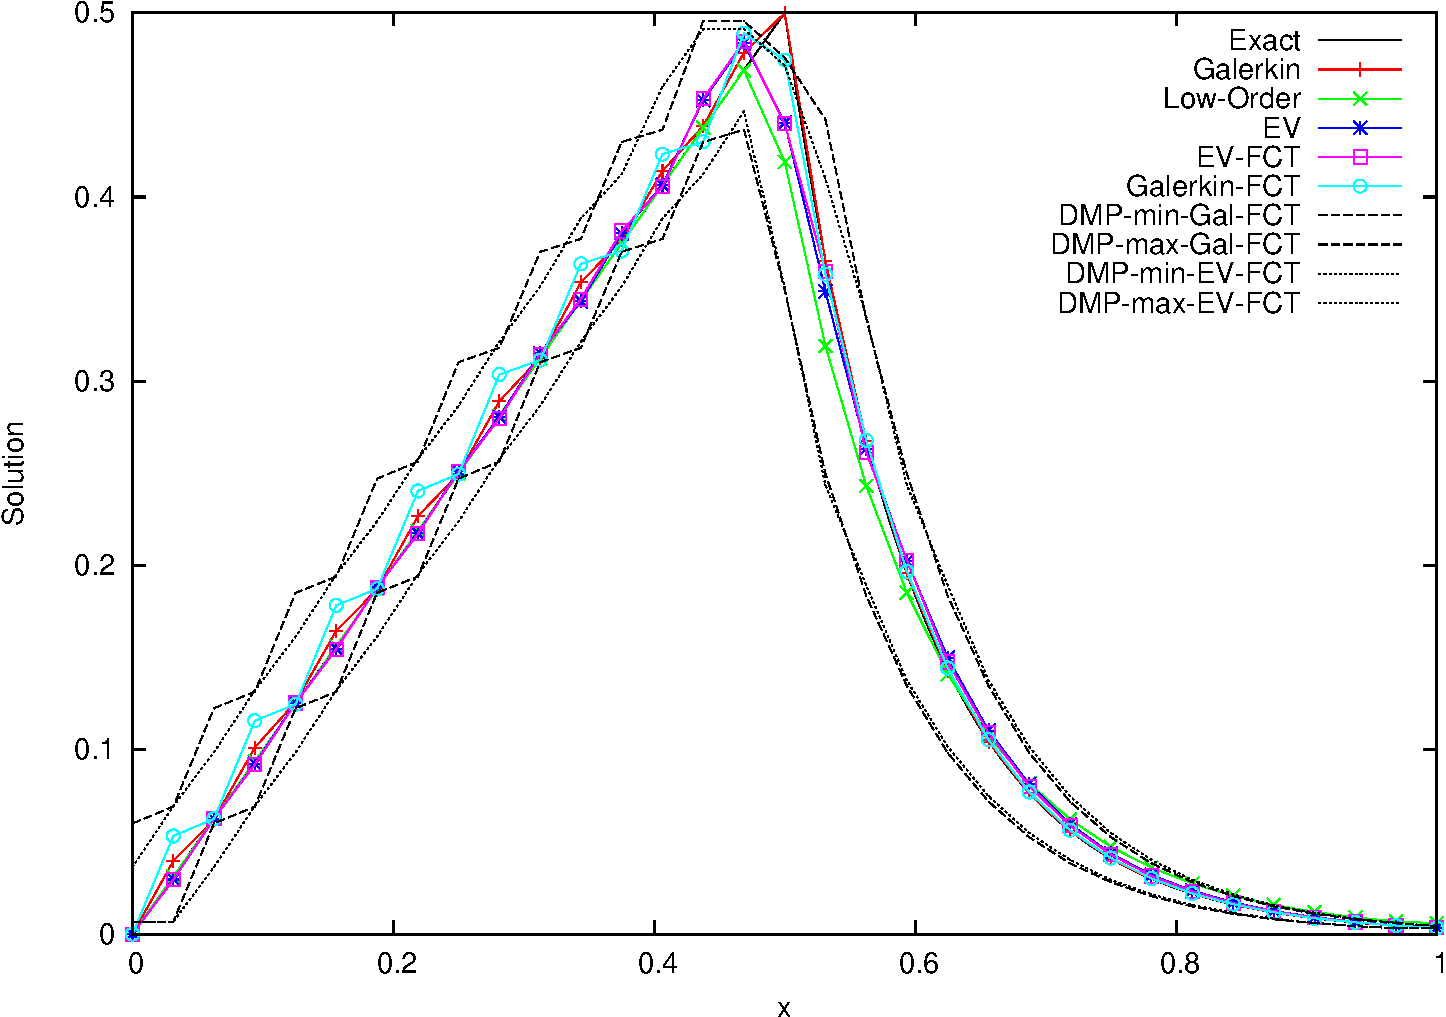
\includegraphics[width=\textwidth]{source_void_to_absorber/coarse.pdf}
   \caption{Comparison of Solutions for Source-Void-to-Absorber Problem
     with $2^5$ Cells}
   \label{fig:source_void_to_absorber}
\end{figure}
%-------------------------------------------------------------------------------
\begin{figure}[h]
   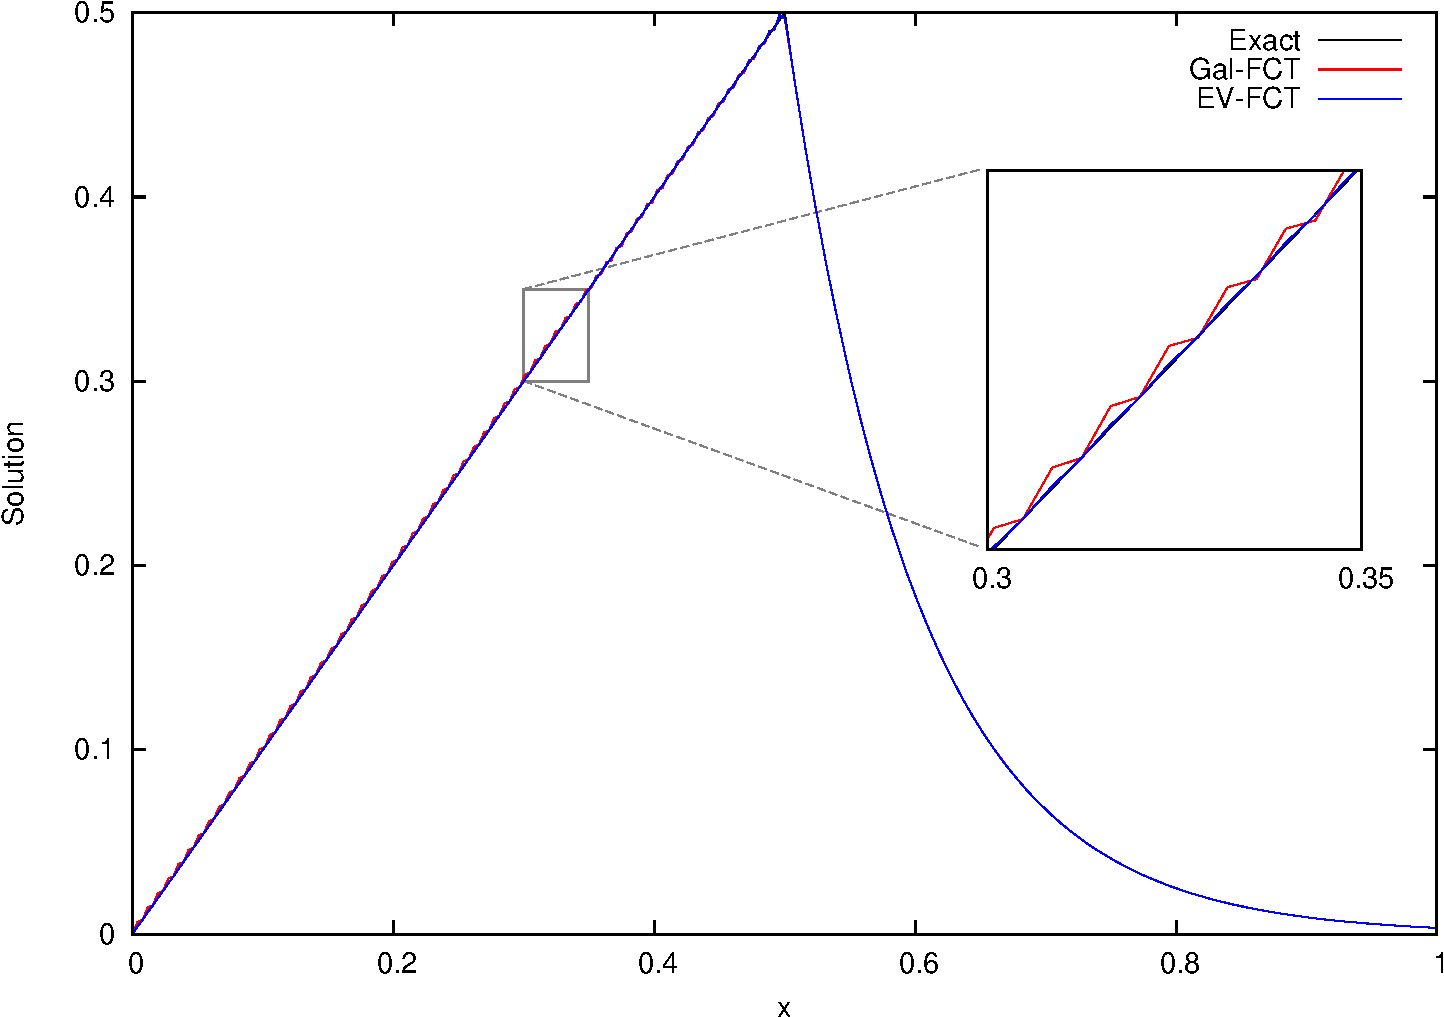
\includegraphics[width=\textwidth]{source_void_to_absorber/fine.pdf}
   \caption{Comparison of Solutions for Source-Void-to-Absorber Problem
     with $2^8$ Cells}
   \label{fig:source_void_to_absorber_fine}
\end{figure}
%-------------------------------------------------------------------------------
\subsection{Code and Version}
Deal.ii code, git commit hash 1bca86bffd5cab926ed3410347bfc7478a18ce8f
